\appendix 

\chapter{Guía de Uso}

En este apéndice, aprenderemos a usar de forma general el proyecto, explicando paso a paso cada funcionalidad, poniendo a prueba algunos casos de uso y examinando la función de cada parte implicada.

\section{Ingreso}

Tras haber explicado todo el proceso de instalación y tecnologías necesarias para montar el proyecto, vamos a explicar como acceder a él. 

Si hemos seguido los pasos previos mostrados en el apartado de instalación, el proyecto ya debería de estar montado, las imágenes en docker ya construidas y la base de datos ya creada y migrada. Para ejecutarlo simplemente desde la carpeta inicial del proyecto abrimos una terminal y escribimos el siguiente comando:

\begin{minted}{bash} 
    $ docker-compose up
\end{minted}

Este comando inicializa los contenedores de docker y ejecuta el proyecto en el entorno local de nuestro ordenador. Para acceder a la aplicación web, debemos de usar un navegador como puede ser Google Chrome y escribimos en el buscador esta dirección : http://localhost:8000/ que abrirá el proyecto en una ventana de nuestro navegador.

Una vez estemos dentro nos aparecerá la vista de inicio de sesión. Como no tenemos usuarios creados, vamos al apartado de registro y creamos un nuevo superusuario con los campos requeridos \textit{\hyperref[fig:vista-registro]{(Figura A.1)}} que constará con los permisos para realizar cambios y administrar los datos. \vspace{1cm}

\begin{figure}[!ht]
    \centering
    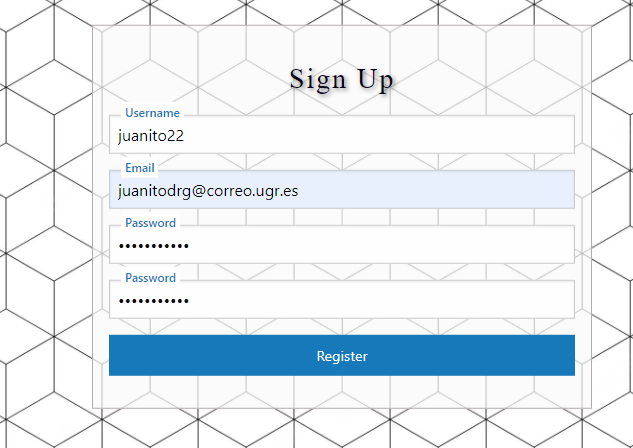
\includegraphics[width=1\textwidth]{imagenes/registro_a.png}
    \caption{ Vista de registro }
    \label{fig:vista-registro}
\end{figure}\vspace{0.5cm}

Una vez registrados, ya podemos hacer login y acceder al panel de administración.\vspace{0.5cm}

\section{Gestión}\vspace{0.5cm}

\subsection{Administración de preguntas}\vspace{0.5cm}

Lo primero de todo es definir las preguntas que queremos que el bot realice a los usuarios. Para ello dentro del apartado de preguntas, en la esquina superior derecha se encuentra la funcionalidad de añadir pregunta. Clicamos y nos abrirá la vista para añadirla. Son necesarios los campos del enunciado y posibles respuestas a la pregunta. 

En la \textit{\hyperref[fig:creacion_pregunta]{Figura A.2}} se ve un ejemplo de una pregunta de prueba que se ha creado. Como vemos se le he asignado cuatro posibles respuestas. Se ha añadido también dos preguntas más, cada una con sus respuestas específicas para que luego se puedan identificar.
\vspace{0.5cm}

\begin{figure}[!ht]
    \centering
    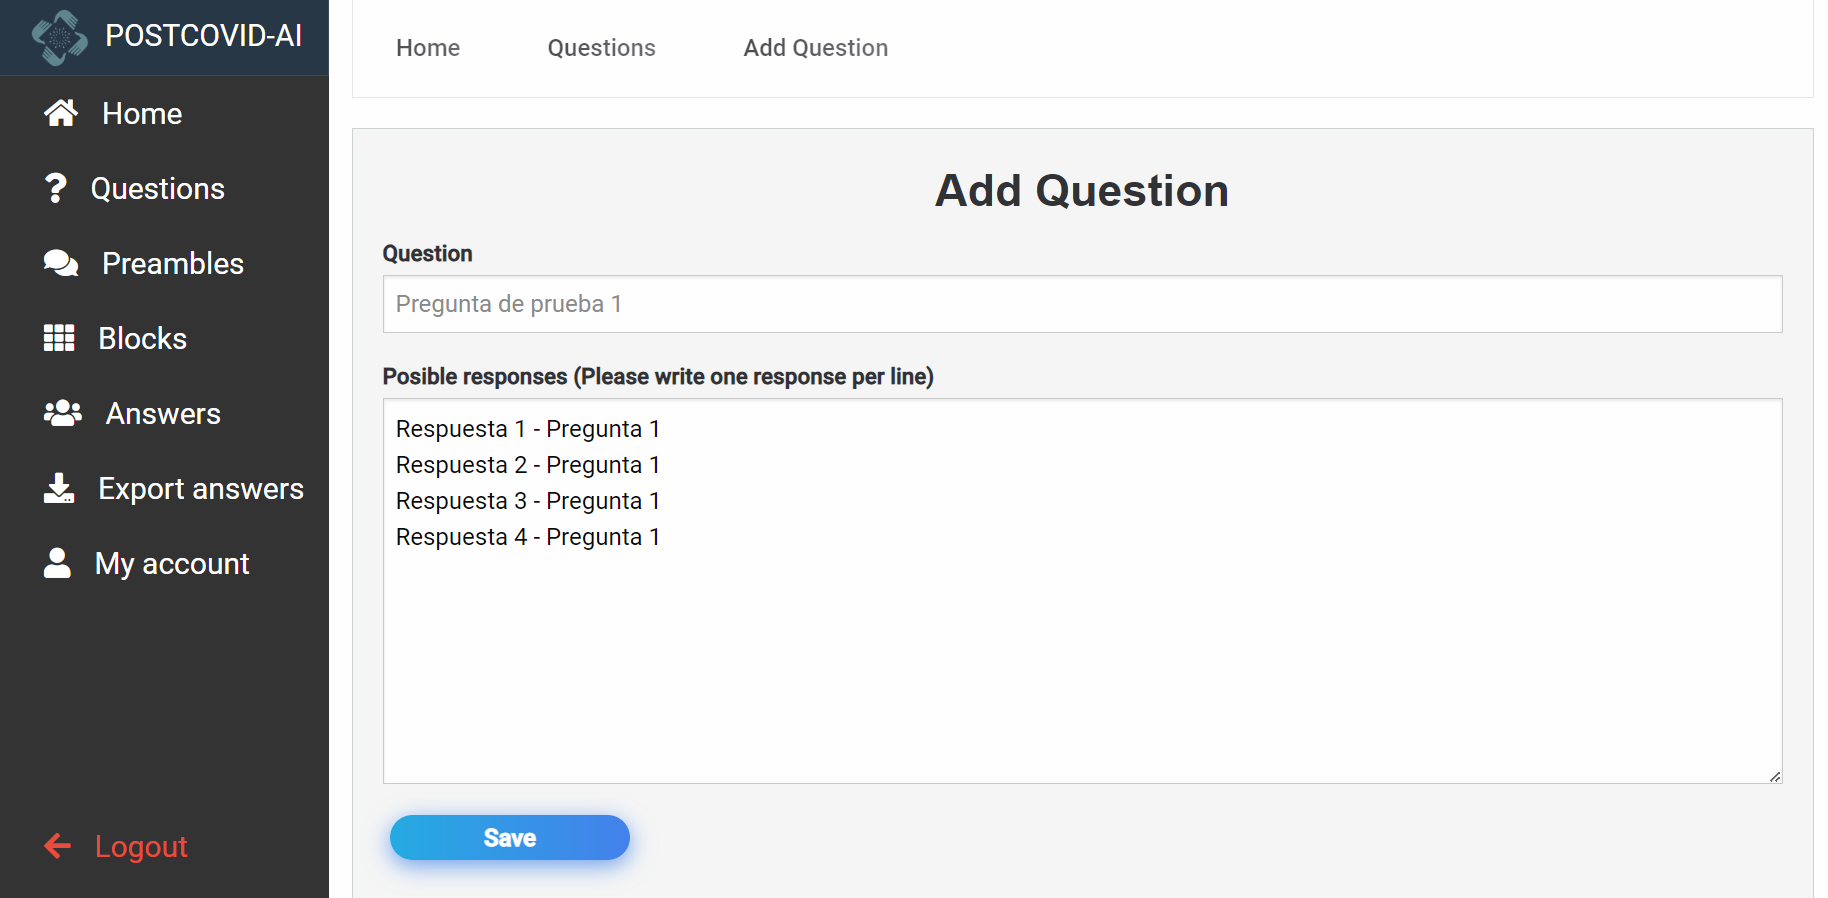
\includegraphics[width=1\textwidth]{imagenes/creacion_pregunta.png}
    \caption{ Vista de creación de pregunta }
    \label{fig:creacion_pregunta}
\end{figure}
 

En la \textit{\hyperref[fig:listado-preg]{Figura A.3}} vemos las tres preguntas que se acaban de crear con algunos datos relevantes. Si desde aquí se clica en la fila de la pregunta se abrirá una vista para modificar la pregunta o si le damos al icono de la papelera, aparecerá un modal para eliminarla.\vspace{0.5cm}

\begin{figure}[!ht]
    \centering
    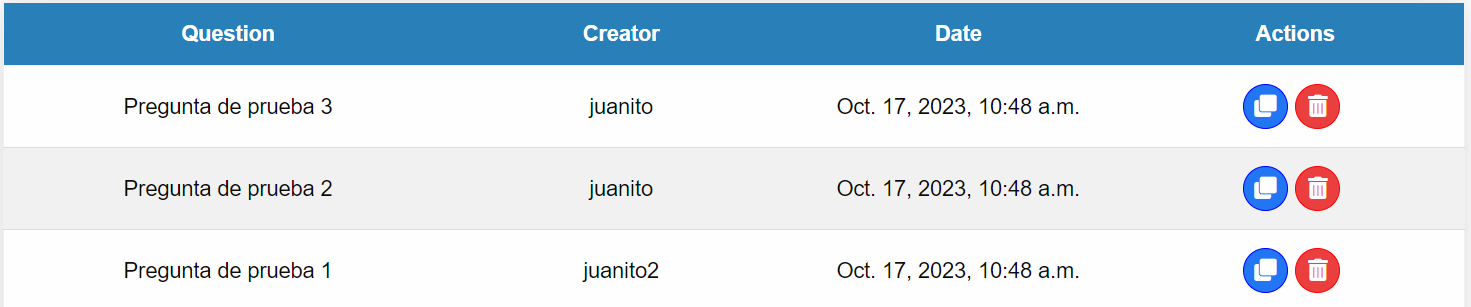
\includegraphics[width=1\textwidth]{imagenes/preguntas_prueba.png}
    \caption{ Vista de listado de preguntas }
    \label{fig:listado-preg}
\end{figure}\vspace{1cm}

\subsection{Administración de Preámbulos}

Aquí se definirán los preámbulos, es decir, los mensajes que mostrará el bot cuando haga el cuestionario asociado a un bloque. Para añadirlo, desde la página principal nos dirigimos al apartado de preámbulos que nos abrirá la vista de los preámbulos registrados y al igual que antes creamos uno. 

Se crea de igual forma que la pregunta como se ve en la \textit{\hyperref[fig:creacion-contexto]{Figura A.4}}, con la diferencia que el primer campo es el nombre del preámbulo y el segundo los mensajes asociados a él. Cada mensaje deberá ocupar una línea diferente en el formulario. \vspace{2cm}

\begin{figure}[!ht]
    \centering
    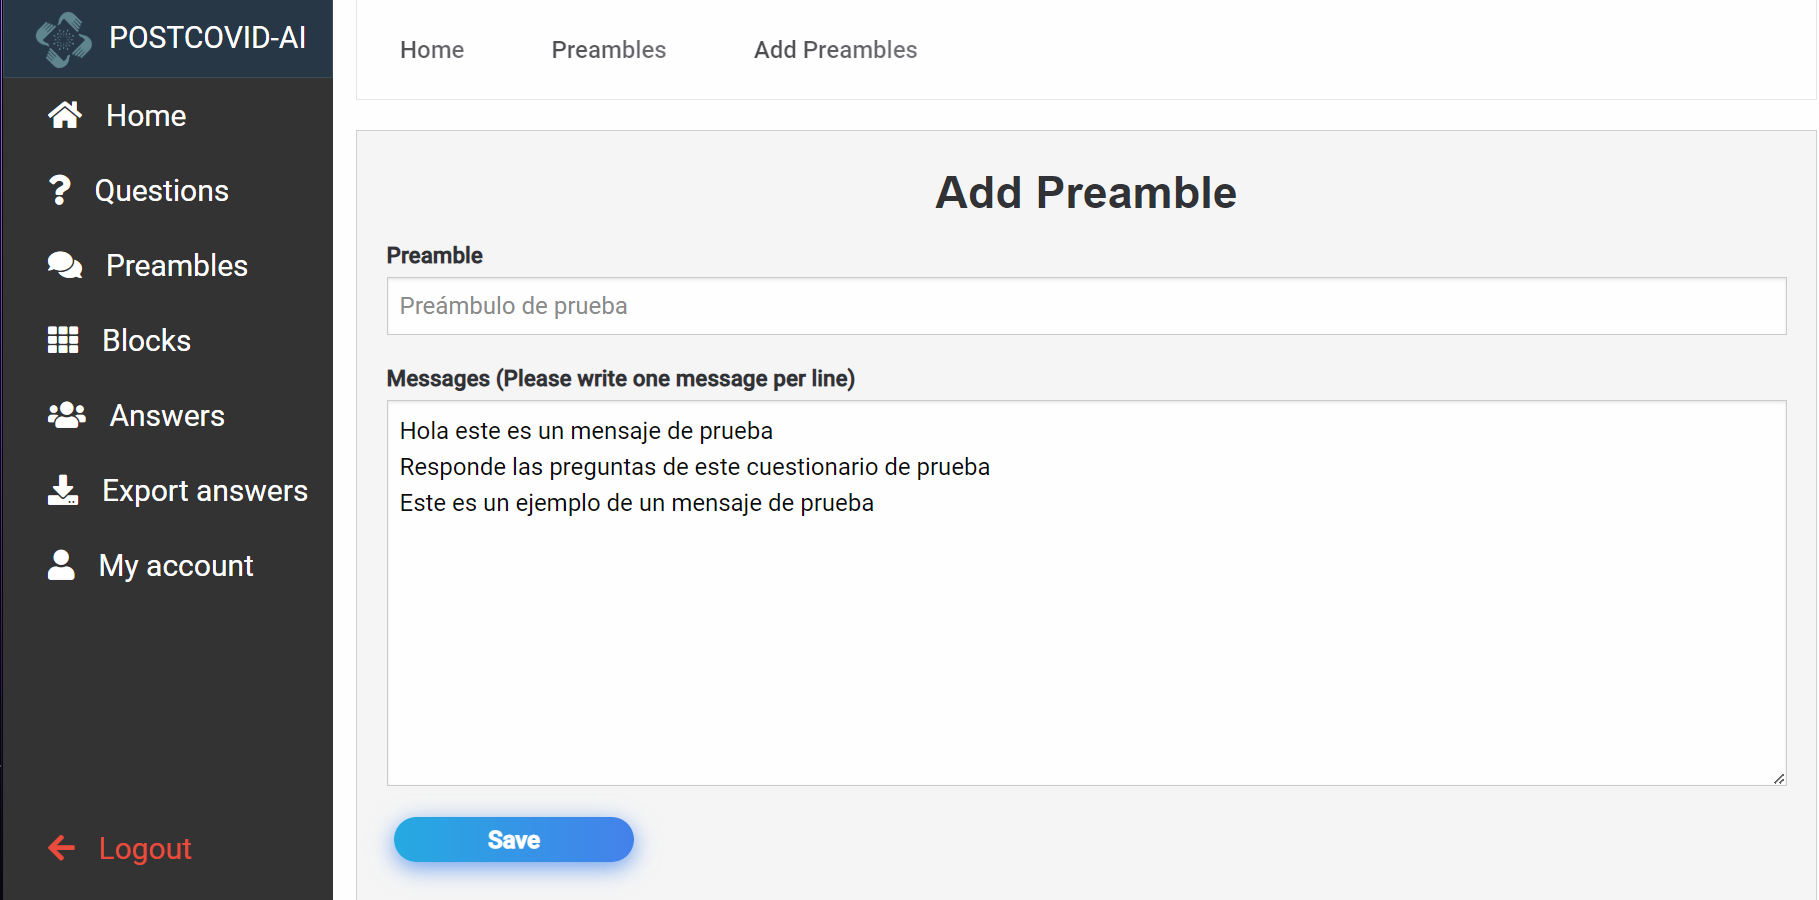
\includegraphics[width=1\textwidth]{imagenes/creacion_preambulo.png}
    \caption{ Vista creación de preámbulo }
    \label{fig:creacion-contexto}
\end{figure}
\vspace{0.5cm}

\subsection{Administración de Bloques}

Pasamos a la creación de bloques. Al igual que en los ejemplos anteriores en el apartado de bloques, podemos añadir nuevos. Elegimos el nombre, las preguntas que queramos que contenga, el preámbulo, elegimos la frecuencia y la planificación \textit{\hyperref[fig:creacion-bloques]{Figura A.5}}. 

\vspace{0.5cm}


\begin{figure}[!ht]
    \centering
    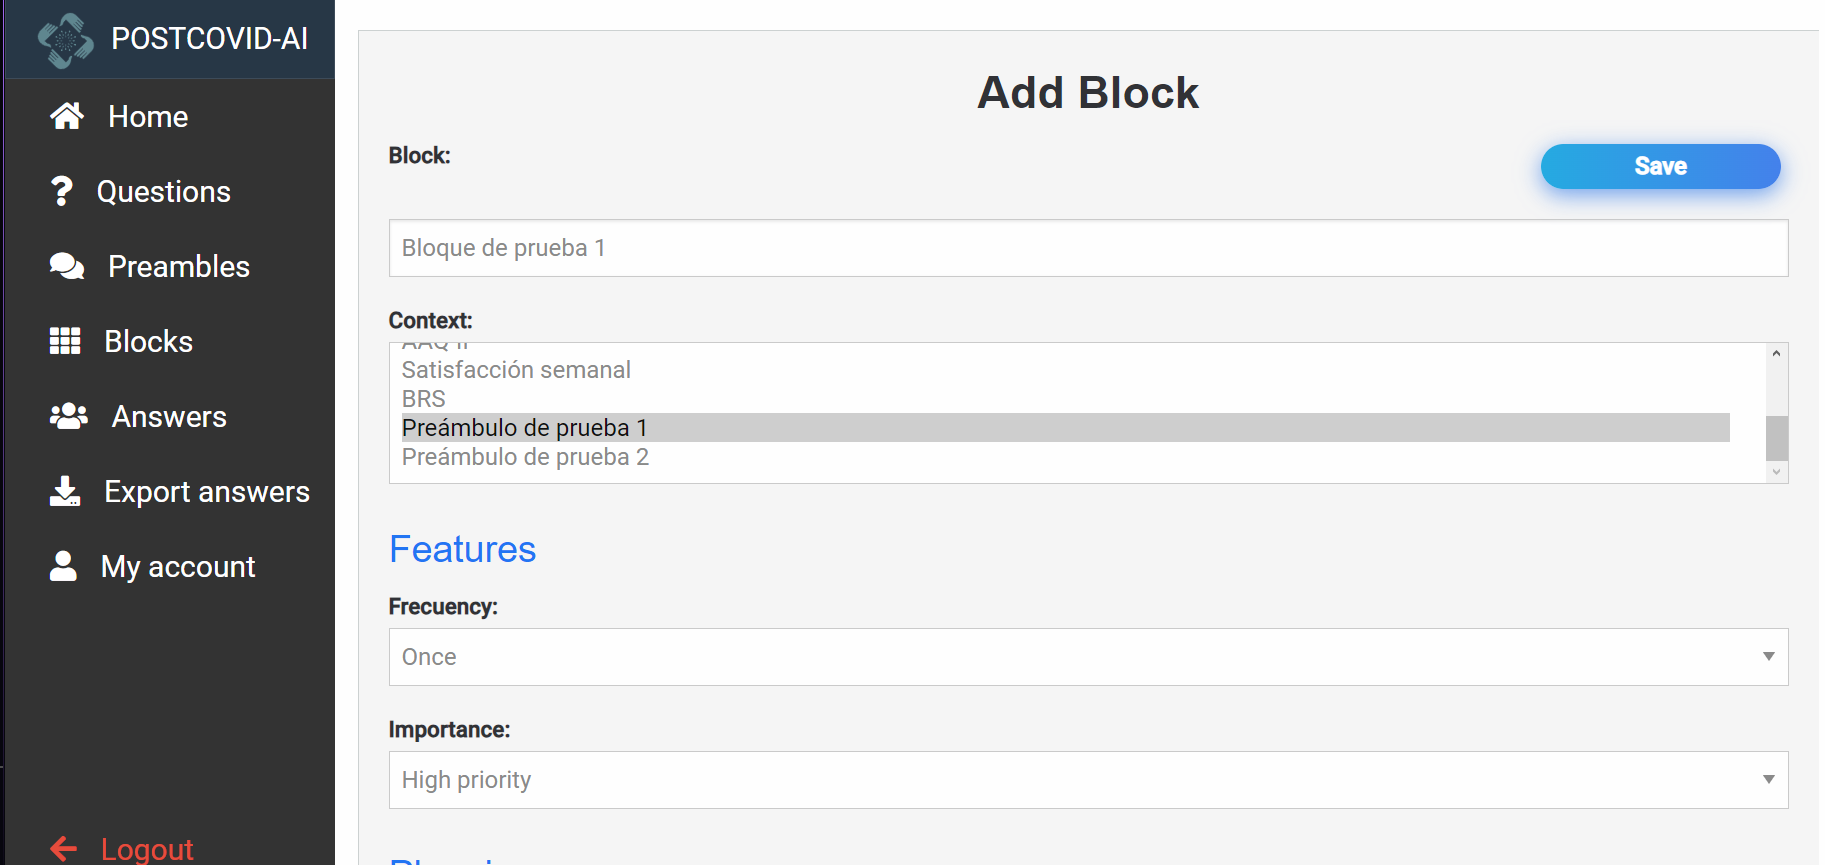
\includegraphics[width=1\textwidth]{imagenes/creacion_bloque1.png}
    \label{fig:creacion-bloques}
\end{figure}\vspace{2cm}

\begin{figure}[!ht]
    \centering
    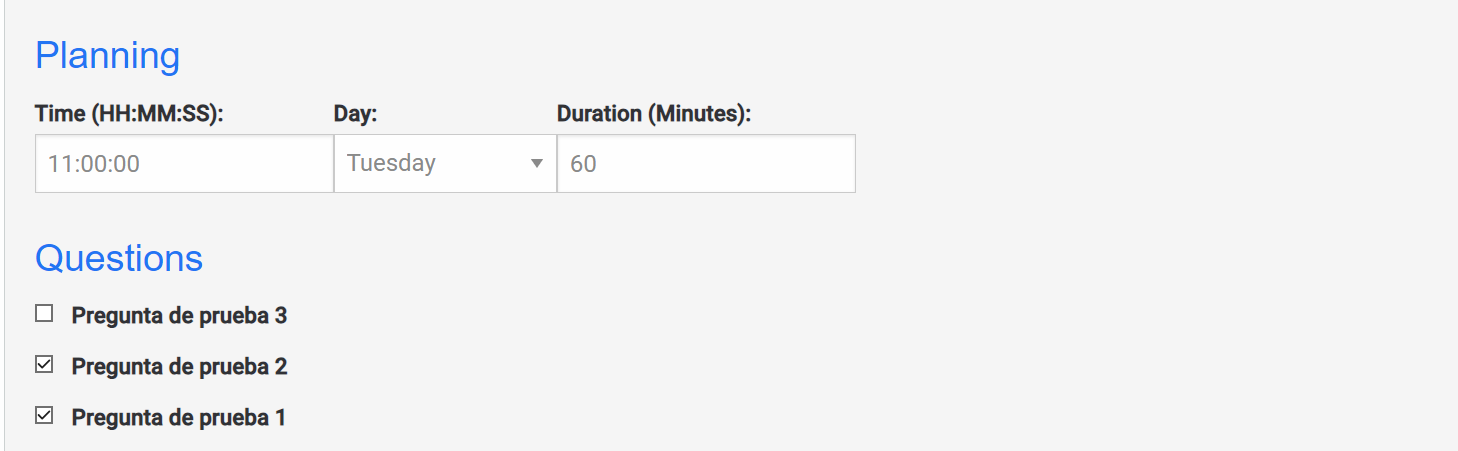
\includegraphics[width=1\textwidth]{imagenes/creacion_bloque2.png}
    \caption{ Vista creación de bloques }
    \label{fig:creacion-bloques}
\end{figure}\vspace{0.5cm}

He creado dos bloques para este ejemplo, como se ve en la \textit{\hyperref[fig:contextos-creados]{Figura A.6}}. Uno con las dos primeras preguntas y el primer preámbulo, y otro con la última pregunta y otro preámbulo.  

\begin{figure}[!ht]
    \centering
    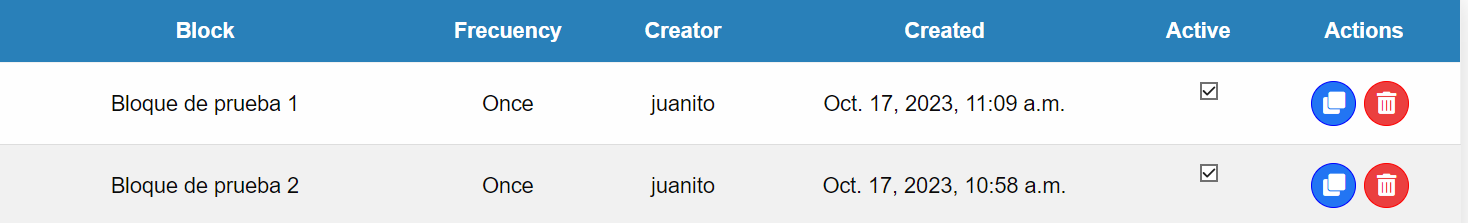
\includegraphics[width=1\textwidth]{imagenes/bloques_prueba.png}
    \caption{ Vista listado de bloques }
    \label{fig:creacion_contexto}
\end{figure}


\subsection{Respondiendo al cuestionario}

Una vez hecho esto, ya podemos pasar a hablar con el bot. Nos dirigimos al chat de Telegram y empezamos la conversación \textit{\hyperref[fig:cuestionario1]{Figura A.7}}.

\begin{figure}[!ht]
    \centering
    
\includegraphics[width=1\textwidth]{imagenes/bot1.png}
    \caption{ Introducción del bot }
    \label{fig:cuestionario1}
\end{figure}\vspace{0.5cm}

El bot detecta que tenemos preguntas pendientes debido a que hemos creado un nuevo bloque y lo hemos planificado para el momento actual, por lo que pasaría a realizar el cuestionario \textit{\hyperref[fig:cuestionario2]{Figura A.8}}. Empieza realizando las preguntas asociadas al último bloque creado. Primeramente muestra uno de los mensajes del preámbulo y realiza la primera pregunta, respondemos y realiza la segunda con sus respuestas correspondientes. Y así con cada uno de los bloques que se encuentren activos. 

\begin{figure}[!ht]
    \centering
    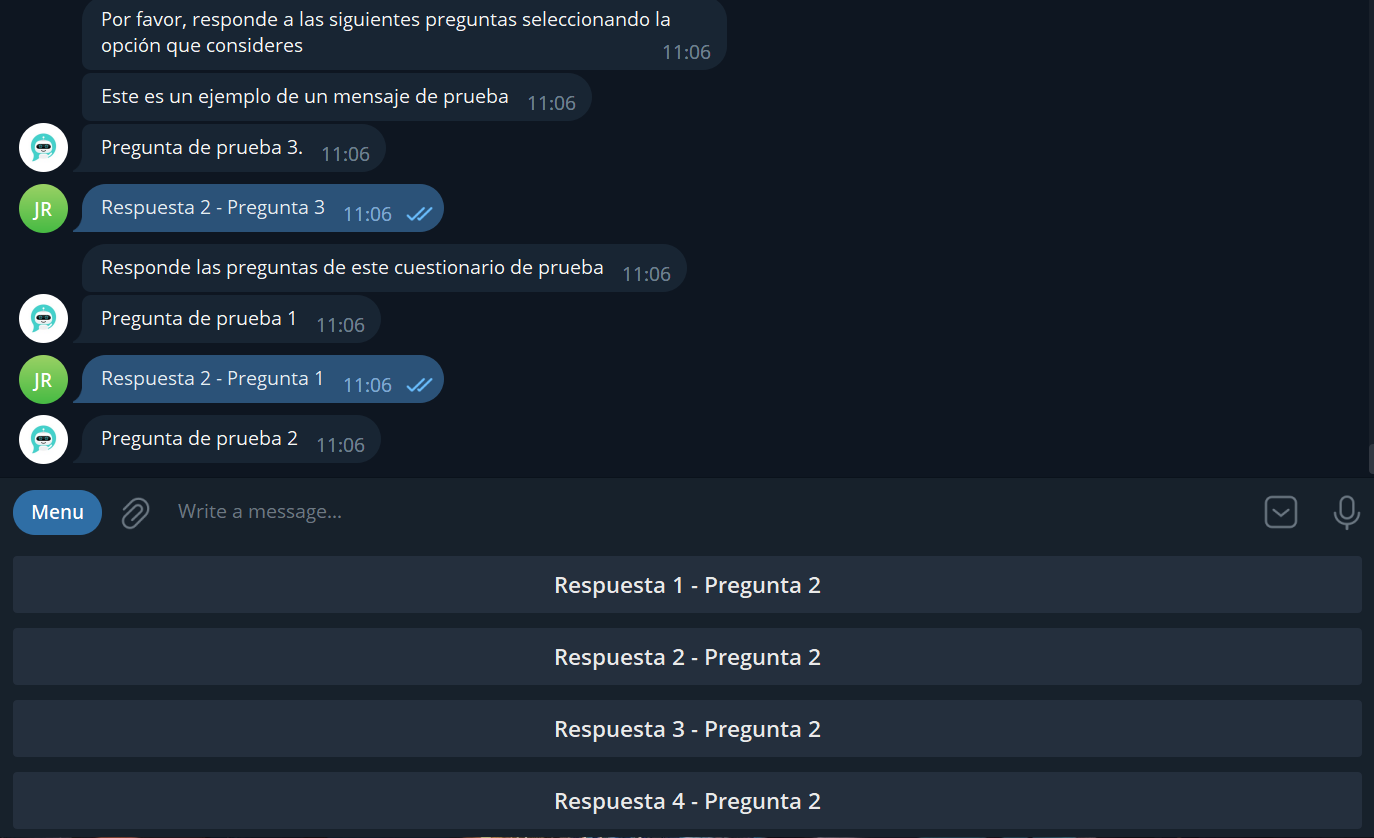
\includegraphics[width=1\textwidth]{imagenes/bot2.png}
    \caption{ Cuestionario }
    \label{fig:cuestionario2}
\end{figure}

Una vez se hayan respondido todas las preguntas, el bot nos informará de que hemos respondido todos los cuestionarios pendientes \textit{\hyperref[fig:cuestionario3]{Figura A.9}}. En este momento es cuando entramos en la sala de espera, en la que podemos tener una conversación con el bot y este avisará al usuario en el momento que otro cuestionario se encuentre activo según las planificaciones.


\begin{figure}[!ht]
    \centering
    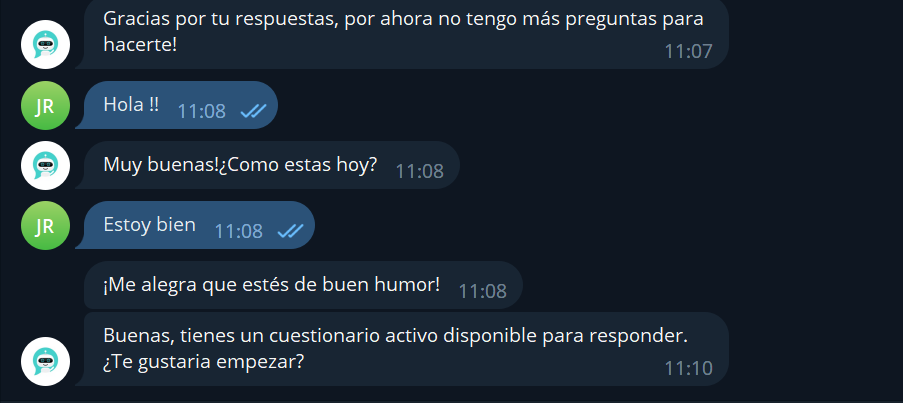
\includegraphics[width=1\textwidth]{imagenes/bot3.png}
    \caption{ Ejemplo de conversación }
    \label{fig:cuestionario3}
\end{figure}\vspace{0.5cm}

\subsection{Administración de Respuestas}

Finalmente, volvemos a la aplicación y esta vez nos dirigimos al último apartado de respuestas. Podemos ver en la \textit{\hyperref[fig:listado_respuestas]{Figura A.10}} que se han generado las repuestas a la preguntas que hemos respondido. 

\begin{figure}[!ht]
    \centering
    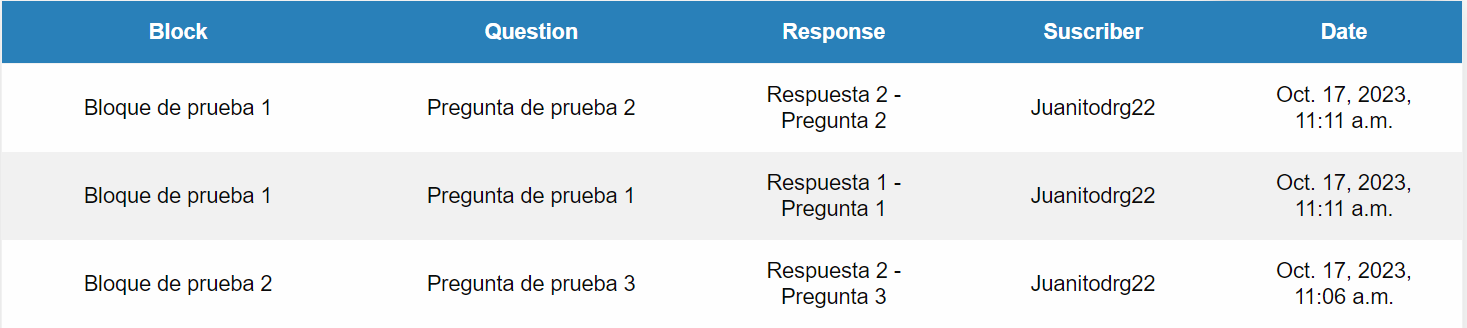
\includegraphics[width=1\textwidth]{imagenes/respuestas.png}
    \caption{ Vista listado de respuestas }
    \label{fig:listado_respuestas}
\end{figure}\vspace{0.5cm}

Si clicamos en el botón de exportar a CSV nos descarga un archivo que contiene ordenado por columnas la información a las respuestas proporcionadas \textit{\hyperref[fig:respuestas-csv]{(Figura A.11)}}. 

\begin{figure}[!ht]
    \centering
    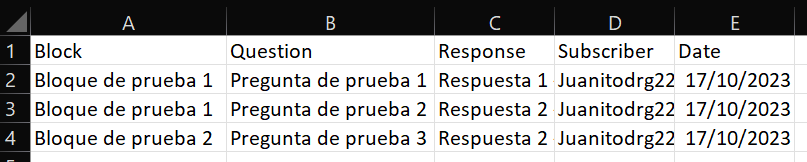
\includegraphics[width=1\textwidth]{imagenes/respuestas_csv.png}
    \caption{ Respuestas CSV }
    \label{fig:respuestas-csv}
\end{figure}\vspace{0.5cm}